\chapter{提案手法}
\label{chap:propose}

\section{データ作成}
本研究では八重山諸島の船舶航路を対象とし、安栄観光\cite{anei}と windy.com\cite{windy}というwebサイトからデータを取得し、機械学習を用いて欠航予測を行うことを目的とする。

\subsection{安栄観光、windy.comからデータの取得}
安栄観光\cite{anei}の運行状況のページから波照間島航路、西表島上原航路、鳩間島航路、西表島大原航路、小浜島航路、竹富島航路、黒島航路の7つの運行状況データを使用する。運行状況データにはそれぞれの航路別で出港時間毎に通常運行、欠航の情報がある。それぞれの航路は図\ref{aneikouro}となる。
\\ windy.com\cite{windy}では地球の任意の地点を選択し、天気予報などの様々な情報を確認することができる。八重山諸島航路は鳥瞰すると西表島と石垣島間を行き来する運行航路であることから、運行航路の北側、南側の2地点からデータを取得する。2地点の風速、最大風速、最大風速の風向、波高、波の向き、うねり、うねりの向き、うねりの間隔の数値データを対象とする。このデータは当日の7時から17時まで2時間間隔で取得し、当日から7日先までは0時から21時まで3時間間隔で確認することができ、当日から8日、9日、10日の3日間は3時から21時までの6時間間隔で確認できるため、以上のデータを取得する。また、気象データとしてWebページのスクリーンショットを当日から9日先までは7時から17時までの2時間間隔で取得し10日先に関しては7時から11時までを取得する。windy.com\cite{windy}ではレイヤーで風速、波高等の情報が分かれているため、その2種類のレイヤーで画像データとして取得する。
\\ 風速、波高データを取得する理由として、対象の航路の欠航判断基準\cite{stan}に風速、波高、視程等の項目があるため、参考にデータの取得範囲を風速、波高等に設定した。
\subsection{データセットの作成}
安栄観光\cite{anei}から得た運行状況データを教師データラベルとして、それ以外のデータを特徴量として機械学習にデータを適用するために前処理を行う。本研究では数値データと画像データを取得しているため、別々のデータセットとしてデータを作成していく。
前処理として取得した運行状況データは運行を0に、欠航を1の二値にエンコードする。画像データは画像を数値に変換するためにRGBの値にエンコードし$64\times64$のサイズにリサイズする。
\\ 例として1便の運行状況データを図\ref{anei_label}の赤枠を1サンプルの教師データとする。特徴量は運行状況データの時間帯周辺で取得された風速、波高等データを合わせたものを数値データのデータセットでは図\ref{value_data}のような例を1サンプルとする。画像データのデータセットでは風速、波高レイヤーでスクリーンショットを行った画像を特徴量とし図\ref{wind_data}、図\ref{wave_data}のように1サンプルとする。これらのサンプルデータの作成方法で数値、画像データを構築する。

\begin{figure}[H]
 \centering
 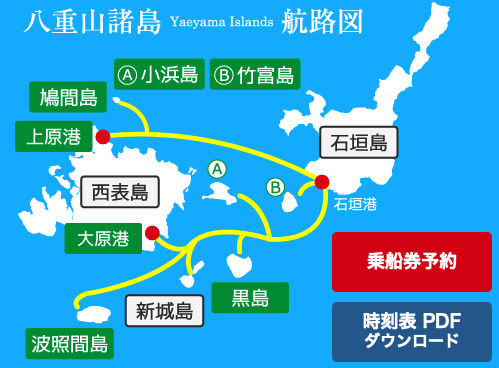
\includegraphics[keepaspectratio, scale=0.5]{fig/chapter3/aneikouro.png}
 \caption{安栄観光\cite{anei}の航路図}
 \label{aneikouro}
\end{figure}

\begin{figure}[H]
 \centering
 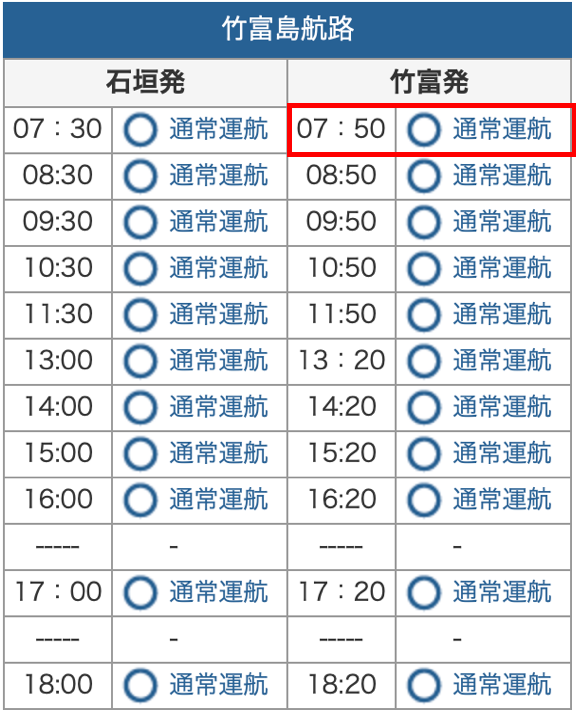
\includegraphics[keepaspectratio, scale=0.7]{fig/chapter3/anei_sample_data.png}
 \caption{安栄観光\cite{anei}の航路便運行状況}
 \label{anei_label}
\end{figure}

\begin{figure}[H]
 \centering
 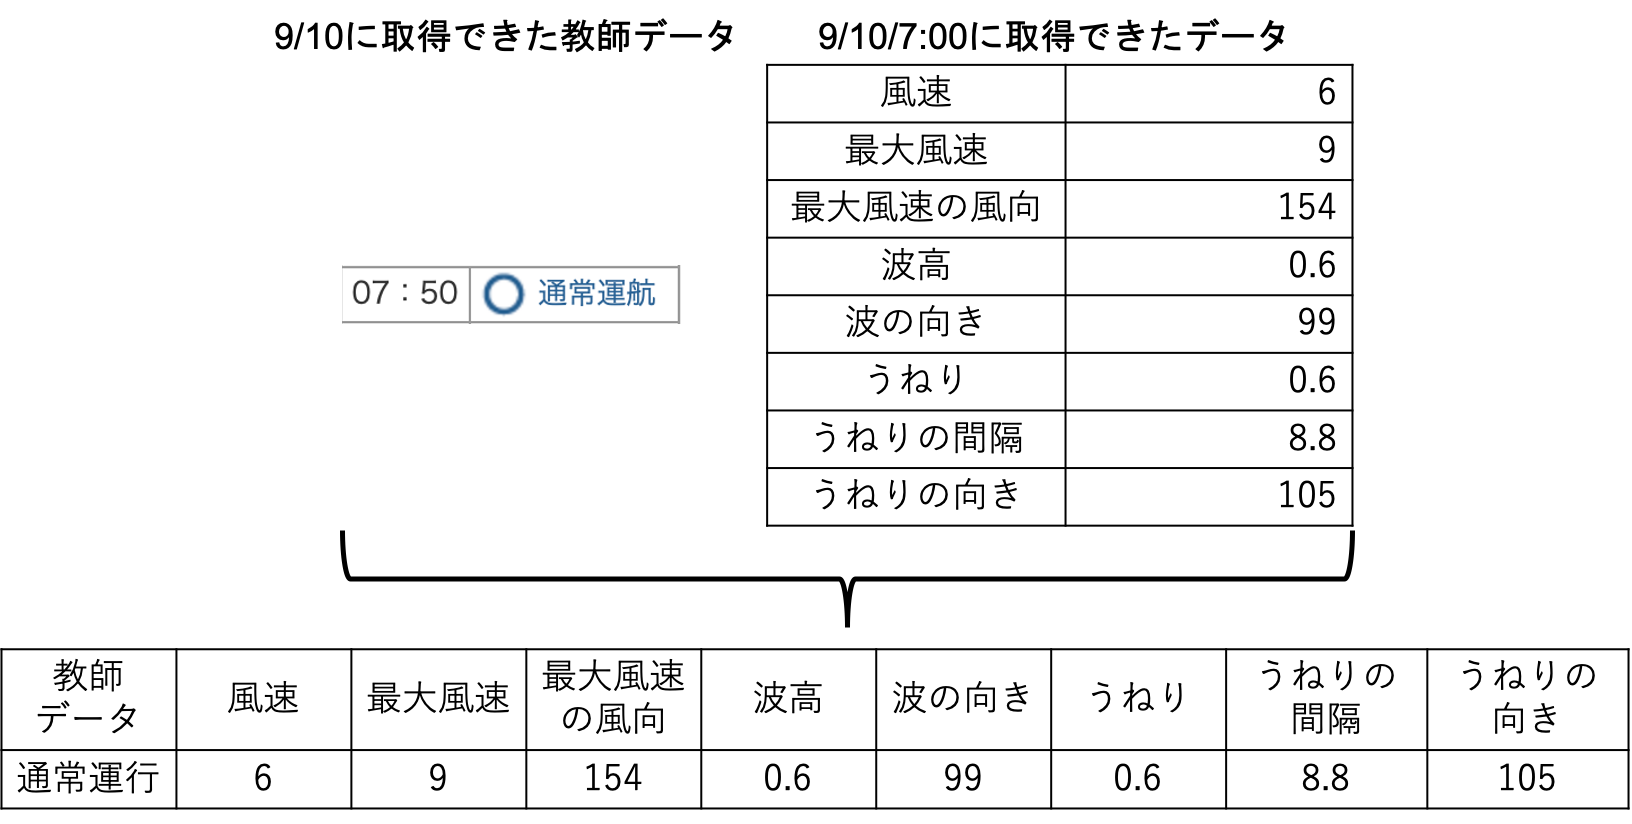
\includegraphics[keepaspectratio, scale=0.5]{fig/chapter3/value_dataset.png}
 \caption{数値データの作成例}
 \label{value_data}
\end{figure}



\begin{figure}[htbp]
 \begin{minipage}{0.5\hsize}
  \begin{center}
   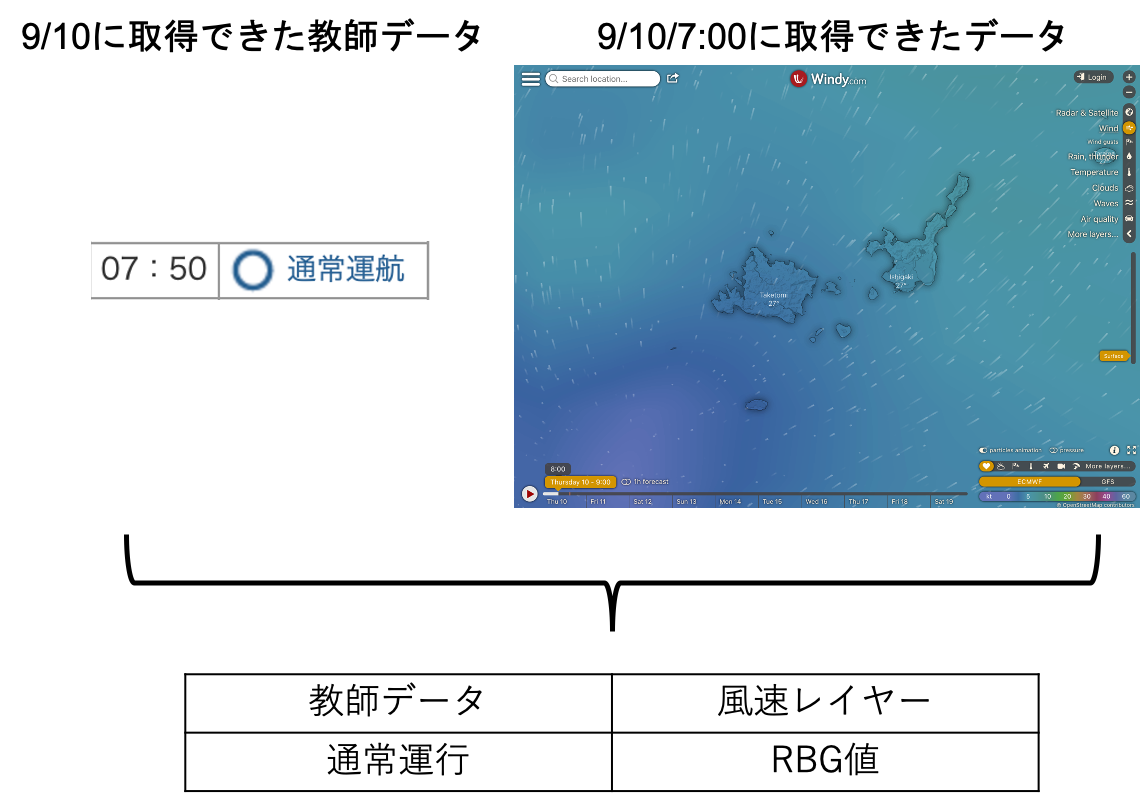
\includegraphics[keepaspectratio, scale=0.38]{fig/chapter3/wind_speed_data.png}
  \end{center}
  \caption{風速画像データの作成例}
  \label{wind_data}
 \end{minipage}
 \begin{minipage}{0.5\hsize}
  \begin{center}
  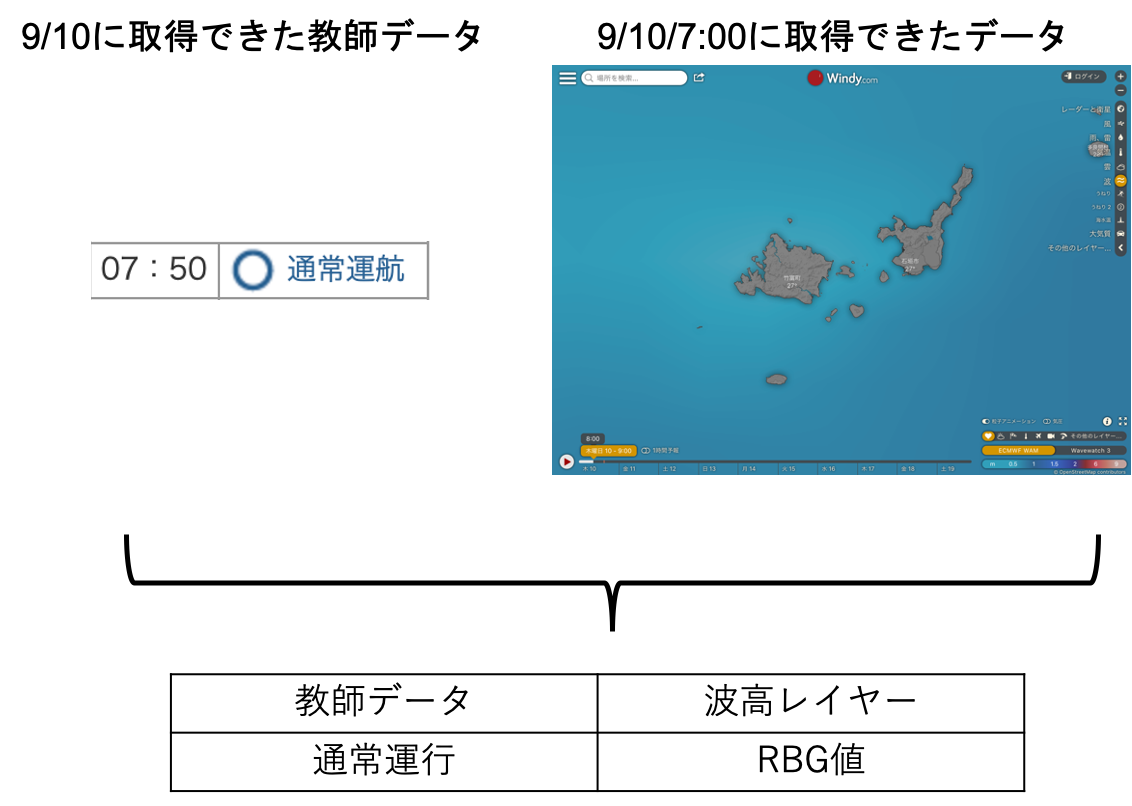
\includegraphics[keepaspectratio, scale=0.38]{fig/chapter3/wave_height_data.png}
  \end{center}
   \caption{波高画像データの作成例}
  \label{wave_data}
 \end{minipage}
\end{figure}

\section{運航状況の分類手法}
本研究では教師あり学習の分類問題として機械学習モデルを適用する。数値データセットではLightGBMを用い、画像データセットでは、CNNを使用する。
\subsection{学習モデル}
実験に使用したデータは大まかに2020年8月から2021年1月までの期間に取得できたものとなる。
学習モデルは航路に特化させるために航路ごとにデータセットを分けて学習を行うことで7航路あるうちのそれぞれに出発港が2つあるため$7\times2=14$個のモデルとなる。さらに、データを教師データの当日から$9=n$日前までの特徴量をスライドさせ当日のデータから当日の予測、n日前のデータからn日後の予測を行うためモデルを分けた。モデルを分けて作成したためモデルの総数は$14\times10=140$とし、数値データは図\ref{value_flow}となる。また画像データではさらに風速レイヤー、波高レイヤーで別々のデータセットのため$140\times2=280$個のモデルがあり、図\ref{img_flow}となる。

\begin{figure}[H]
 \centering
 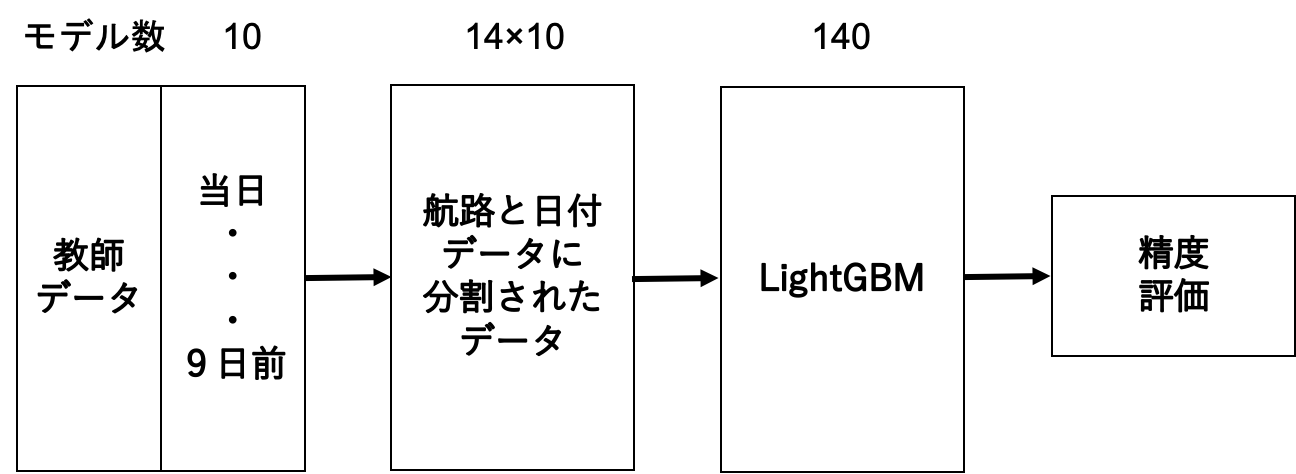
\includegraphics[keepaspectratio, scale=0.5]{fig/chapter3/value_flow.png}
 \caption{数値データの学習フロー}
 \label{value_flow}
\end{figure}

\begin{figure}[H]
 \centering
 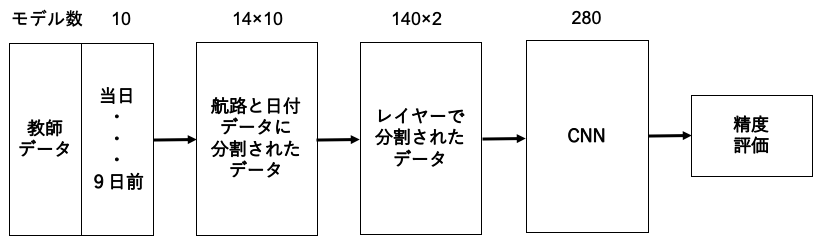
\includegraphics[keepaspectratio, scale=0.5]{fig/chapter3/img_flow.png}
 \caption{画像データの学習フロー}
 \label{img_flow}
\end{figure}





